\section{Modifying and applying RISE (Single Pixel)}
\nblink{brats/06\_rise.ipynb}

apply on a single pixel, pixel == class

\subsection{Results}

\begin{figure}[H]
\centering
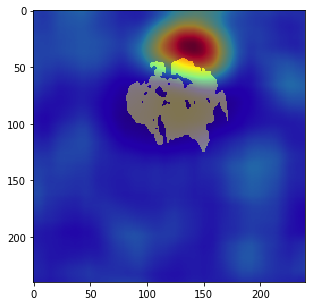
\includegraphics[width=5cm]{chapters/04_segmentation/images/rise_single_pixel.png}
\caption{Extracted horizontal slices with merged tumor segment}
\end{figure}



\subsection{Discussion}

\subsection{Conclusion}
Works, but low resolution even with 3000 masks

\section{Modifying and applying RISE (Multi Pixel)}
\nblink{17\_rise\_multipixel.ipynb}


\begin{figure}[H]
    \centering
    \caption{RISE Multipixel (Mean)}
    \begin{subfigure}{.5\textwidth}
        \centering
        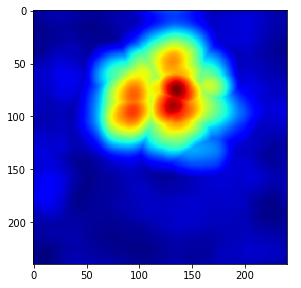
\includegraphics[width=5cm]{chapters/04_segmentation/images/rise_multipixel_max_1-0.png}
        \caption{ the text for a}
    \end{subfigure}%
    \begin{subfigure}{.5\textwidth}
        \centering
        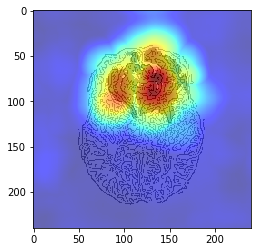
\includegraphics[width=5cm]{chapters/04_segmentation/images/rise_multipixel_max_1-1.png}
        \caption{b}
    \end{subfigure}
    \caption{Explanation text}
\end{figure}

\subsection{Results}

\subsection{Discussion}

\subsection{Conclusion}
